% !TEX root = ../thesis_main.tex



%%%% --- * --- %%%%	
\clearpage
%\chapter{Introduction}
\chapter{Background}
\label{intro_chapter}
\label{nuclear_chapter}
The nuclear weak force is one of four fundamental forces described within physics.  It mediates the process of beta decay, which is of particular interest to us here.  Although beta decay is generally well understood, it presents a unique opportunity for precision measurements to search for physics beyond the Standard Model within the Weak coupling.  By observing the kinematics and angular correlations involved in the decay process, one gains access to a wealth of information about the form of the operators mediating the decay.  

\section{Beta Decay within the Standard Model}
A nucleus undergoing beta decay converts one of its protons (neutrons) into a neutron (proton), and simultaneously emits a lepton and anti-lepton.  The daughter nucleon remains bound in place of its parent, and the overall electric charge of the nucleus is changed by -1 (+1), with the extra charge being carried away by the anti-lepton (lepton).  In particular, at the nucleon level, three beta decay processes are possible:
\bea
	p &\rightarrow& n + e^+ + \bar{\nu}_e  \label{eq:betaplus_decay} \\
	n &\rightarrow& p + e^- + \nu_e, \label{eq:betaminus_decay}  \\
	p + e^- &\rightarrow& n + \nu_e \label{eq:electroncapture}
\eea
where the processes described in Eqs.~\ref{eq:betaplus_decay} and~\ref{eq:electroncapture} are energetically disallowed for an unbound proton, however there is no similar requirement for Eq.~\ref{eq:betaminus_decay}.  

Limiting the focus of this discussion to Eq.~\ref{eq:betaplus_decay}, we note that this expression provides no information at all about the momenta or spin of the outgoing daughter particles.  This behaviour is governed by the form of the Weak coupling that mediates the decay.  

Within the field of nuclear physics, it is common to classify beta decay processes as being either ``Allowed'' or ``Forbidden'' (sometimes with an associated number to describe the extent to which it is Forbidden), where Forbidden processes are generally suppressed but not truly forbidden.  In an Allowed transition, the positron and anti-neutrino are treated as being created at the nuclear centre, and as a result they may not carry away any \emph{orbital} angular momentum.  However, since the outgoing leptons both have spin $S=1/2$, it is still possible for the total nuclear angular momentum, $J$, to be changed in an Allowed decay.  This implies that an Allowed transition must \emph{always} change the total nuclear angular momentum by either $0$ or $\pm1$.  

The Allowed decays traditionally are further separated into a ``Fermi'' singlet in which the two leptons have anti-parallel spins and there is no change to nuclear angular momentum ($\Delta J = 0$), and a ``Gamow-Teller'' triplet, where the two lepton spins are aligned in parallel to one another and so the \emph{projection} of the nuclear angular momentum is changed by $\pm1$.  This implies that the total nuclear angular momentum is changed by $\Delta J = \{0, \pm1\}$ during a Gamow-Teller transition.  A mixed transition is also possible, however we note that the $J_i = J_f = 0$ decays must always be pure Fermi transitions, because there is no way to produce this result from two outgoing leptons with parallel spins.~\cite{krane}~\cite{wong1990}~\cite{severijns_beck_cuncic_2006}.

Given the differing behaviour within the angular momenta of the daughters in Fermi and Gamow-Teller transitions, it is perhaps not suprising that that the \emph{linear} momenta of the outgoing particles should also follow a different set of distributions in these two cases.  At the level of the Weak coupling, Fermi- and Gamow-Teller transitions are governed by different operators, with the Fermi interaction mediated by a so-called ``vector'' ($V$) coupling, and the Gamow-Teller interaction mediated by an ``axial-vector'' ($A$) coupling.



% and therefore carry angular momentum, the total nuclear angular momentum may still be changed.
%Allowed transitions, in which the decay may not  as either ``Fermi'' decays, 
%Since the topic of this work involves the Beta+ decay process of Eq.~\ref{eq:betaplus_decay}, that will be the primary focus in the discussion of beta decay that follows.
%we will focus primarily on that in the discussion that follows.
%We will focus primarily on the process of Eq.~\ref{eq:betaplus_decay}


%%\note{The TRIUMF Neutral Atom Trap (TRINAT) offers an experimental set-up which is uniquely suited to precision tests of Standard Model beta decay physics.  Radioactive ions are delivered from the ISAC beamline and neutralized before being trapped in the first of two magneto-optical traps (MOTs).  Approximately once per second, atoms from the first MOT are transferred to the second, where their decay products can be observed with significantly less background than would have been possible in the first trap (see Figure~\ref{fig:doublemot}).  The transfer methodology is discussed in some detail in a paper by Swanson et al~\cite{swanson}. (The point is that this eliminates background from the decays of other stuff.  Or the same stuff.  Stuff that's not centered at the trap.)}

%\note[color=jb]{JB on the contents of Chapter 1:  \\
%Move what you have in 1.1 and 1.3 to the first section of Chapter 2, and otherwise omit Chapter 1.}


% ~\cite{wu}
% ~\cite{LeeYang}
%\aside{Did I even get this right?  Is the phase angle really what makes it left-handed? \\ JB says:  \\ ... \\ Relative sign.  look at the quark-lepton Lagrangian, which has $(1 \pm \gamma_5)$ } 
%Any such behaviour, should it be present, would necessarily be a non-dominant contribution to the interaction, however it cannot be entirely ruled out.  
%Any such behaviour with would necessarily be only 
% cannot be entirely ruled out, and the search for physical interactions beyond the Standard Model (BSM) is an active field of research. \aside{cite someone?}  
%, and our observable is mostly sensitive to scalar (S) and tensor (T) couplings.  
%\note{According to present limits, these couplings would have to be pretty small relative to the ($V$) and ($A$) couplings.}


%%%%%\note[color=jb]{from JB on the contents of Chapter 1:
%%%%%%\\
%%%%%%With three changes:
%%%%%%\\ ... \\
%%%%%%1)"and we shall be interested especially in scalar (S) and tensor (T) couplings." -> "our observable is mostly sensitive to scalar (S) and tensor (T) couplings."
%%%%%\\ ...\\
%%%%%2)
%%%%%"These couplings all refer to parameters in a Lagrangian that takes the
%%%%%relativistic inner product of a current for the lepton with a current for the
%%%%%proton or neutron.
%%%%%The resulting Lagrangian must be a scalar under Lorentz transformations, so
%%%%%these currents must have transformations like these V,A,S, and T and be
%%%%%combined into a scalar."
%%%%%\\...\\
%%%%%3) Add one reference to the latest review:
%%%%%\\
%%%%%Adam Falkowski, Martín González-Alonso, Oscar Naviliat-Cuncic. Comprehensive analysis of beta
%%%%%decays within and beyond the Standard Model. Journal of High Energy Physics, Springer, 2021, 04,
%%%%%pp.126. 10.1007/JHEP04(2021)126.
%%%%%\\
%%%%%Here it is!~\cite{Falkowski2021}.
%%%%%\\ ... \\
%%%%%You have time for nothing else.
%%%%%}

%%%%%\note[color=jb]{Me:  \\ Is a `phase angle' really what makes it left-handed? \\.\\ JB says:  \\ Relative sign.  look at the quark-lepton Lagrangian, which has $(1 \pm \gamma_5)$ }

%%%%%\bluetodo{Need to figure out how the exotic couplings actually work, mathematically.  What the fuck does ``$(V-A)$'' even *mean*?  IIRC John wants a brief mention of $\gamma_5$'s and $\gamma_\mu$'s, and probably a brief mention of whatever mumble-mumble group is mumble-mumble represented or something.
%%%%%\\
%%%%%...
%%%%%\\
%%%%%JB says:
%%%%%\\
%%%%%the current transforms like a Lorentz scalar or tensor -- this does not refer to the angular momentum.
%%%%%\\
%%%%%If you write down the Lagrangian for beta decay, that's eough. All these things refer to the structure of the Lagrangian. The theory considers all possible Lorentz transformations of the currents. 
%%%%%\\
%%%%%Please don't talk about SU(2)xU(1) for electroweak unification. It's textbook material that's beyond the scope.
%%%%%}

%%%%%%\note{ The general form of the weak interaction Hamiltonian is: \\
%%%%%%\bea
%%%%%%\hat{H}_{\mathrm{weak}} &=& \sum_{i=S,P,V,A,T} \left( {\bar{\psi}}_p {\mathcal O}^i \psi_n \right) \left( C_i \bar{\psi}_e {\mathcal O}_i \psi_\nu + C_i^\prime \bar{\psi}_e {\mathcal O}_i \gamma^5 \psi_\nu \right) + H.C.
%%%%%%\eea
%%%%%%with
%%%%%%\bea
%%%%%%{\mathcal O}_S &=& 1            \\
%%%%%%{\mathcal O}_P &=& \gamma^5     \\
%%%%%%{\mathcal O}_V &=& \gamma_\mu    \\
%%%%%%{\mathcal O}_A &=& i \gamma_\mu \gamma^5  \\
%%%%%%{\mathcal O}_T &=& \frac{-i}{2\sqrt{2}} \left( \gamma_\mu \gamma_\nu - \gamma_\nu \gamma_\mu \right)
%%%%%%\eea
%%%%%%\\
%%%%%%It's from here:  ~\cite{hong_sternberg_garcia}.
%%%%%%\\ 
%%%%%%Also, unclear what subscripts $p,n,e,\nu$ mean.  I could guess/assume, but....
%%%%%%}



%%%% --- * --- %%%%	
%
%
%
%
%
%
%
%%%% --- * --- %%%%	
%\section{Motivation}
\section{A Generalized Description of the Weak Interaction}
%\section{Background}
%\section{Motivation}
%\greycomment{The nuclear Weak force is one of four fundamental forces described within physics.  It mediates the process of beta decay, which is of particular interest to us here.  Although beta decay is generally well understood, it presents a unique opportunity for precision measurements to search for physics beyond the Standard Model within the Weak coupling.  By observing the kinematics and angular correlations involved in the decay process, one gains access to a wealth of information about the form of the operators mediating the decay.}

According to the predictions of the Standard Model (SM), the Weak force involves only vector ($V$) and axial-vector ($A$) couplings, where a relative sign within the quark-lepton Lagrangian produces the left-handed ``$(V-A)$'' form of the interaction in maximal violation of parity.  In terms of physical behaviour, one consequence of this model is that ``regular matter'' leptons emerge from a Weak interaction with left-handed chirality, while antimatter leptons emerge with right-handed chirality. Any deviation from this behavior would be indicative of ``new'' or ``exotic'' (i.e., not previously discovered) physics.  

There exists an extensive body of experimental evidence to demonstrate that the above model is overall a very good description of the beta decay process~\cite{wu}.  Despite the success of the $(V-A)$ model, there are still certain lingering questions that must be addressed by precision measurements.  Any deviation from maximal parity violation (i.e., a ``$(V+A)$'' contribution to the Weak force) would be of great interest to the community, as would the presence of certain other exotic couplings, such as the so-called Scalar ($S$) and Tensor ($T$) interactions.  Any such behaviour beyond the Standard Model (BSM) would represent a non-dominant contribution to the interaction, however the possibility cannot be entirely ruled out.  

%Lee-Yang 
The generalized nucleon-level Lagrangian to describe the Weak interaction including BSM behaviour is given by:
% !TEX root = ../thesis_main.tex
%%%% --- * --- %%%%	
\bea
{\mathcal L} &=& - \bar{p}\gamma^\mu n \left( C_V^+ \bar{e} \gamma_\mu \nu_L + C_V^- \bar{e} \gamma_\mu \nu_R \right) -\bar{p}\gamma^\mu \gamma_5 n \left( C_A^+ \bar{e} \gamma_\mu \nu_L - C_A^- \bar{e} \gamma_\mu \nu_R \right) 
\nonumber\\
&& - \bar{p} n \left( C_S^+ \bar{e} \nu_L + C_S^- \bar{e} \nu_R \right) - \frac{1}{2} \bar{p} \sigma^{\mu\nu} n \left( C_T^+ \bar{e} \sigma_{\mu \nu} \nu_L + C_T^- \bar{e} \sigma_{\mu\nu} \nu_R \right) 
\nonumber\\
&& + \bar{p}\gamma_5 n \left( C_P^+ \bar{e} \nu_L - C_P^- \bar{e} \nu_{R} \right) + \textrm{H.C.}, 
\label{eq:lee_yang_lagrangian} 
\eeawhere the coupling constants $C_X^{\pm}$ (with $X=\{V,A,S,T,P\}$) are written in such a way as to separate out the left-handed ($C_X^{+}$) and right-handed ($C_X^{-}$) components from one another, and the neutrino fields $\nu_{L,R}$ are given a similar treatment.  
%the left- and right-handed components of both the coupling constants and neutrino fields are separated out from one another, with left-handed couplings $C_X^{+} = $
%coupling constants $C_X^{\pm}$ are written
%$C_X^{+}$ and $C_X^{-}$ describe the left-handed and right-handed (respectively) 
A simple variable transform relates Eq.~\ref{eq:lee_yang_lagrangian} to expressions that are potentially more familiar from the older literature, much of which was written before it had been determined that the Weak force is primarily or entirely left-handed: 
\bea
\nu_{L} &=& \frac{1}{2}\nu \left( 1 + \gamma_5 \right) \\
\nu_{R} &=& \frac{1}{2}\nu \left( 1 - \gamma_5 \right) \\
C_X &=& \frac{1}{2} \left( C_X^+ + C_X^- \right) \\
C_X^\prime &=& \frac{1}{2} \left( C_X^+ - C_X^- \right)
\eea
It can be seen from the form of the Lagrangian that the $V,A,S,T,P$ couplings within are described as such because they \emph{behave} as vectors, axial-vectors, scalars, tensors, and pseudoscalars (respectively) under a Lorentz transform, where the Lagrangian itself must be a scaler both before and after a Lorentz transform~\cite{LeeYang}~\cite{Falkowski2021}.


\note[color=bluetodo]{Seriously, this section needs some citations.  Notably, C.S. Wu~\cite{wu} (done) and Lee+Yang~\cite{LeeYang} (done).  Perhaps also Hong+Sternberg+Garcia~\cite{hong_sternberg_garcia}.  Probably a bunch more people too though.}
\note{Write a paragraph about what we're looking for with this experiment.}
%\note[color=done]{John wanted this change (now implemented), but I think the phrasing is unclear now: \\
%"and we shall be interested especially in scalar ($S$) and tensor ($T$) couplings." -> "our observable is mostly sensitive to scalar ($S$) and tensor ($T$) couplings."
%\\ ... \\
%In fact, that sentence is gone now, but I no longer talk about which things we're sensitive to in this section of the intro.}
\note[color=jb]{JB on intuitive concepts that are missing:  
\\
The SM couples to left-handed neutrinos and right-handed antineutrinos. Since the neutrinos only have weak interactions, there are no right-handed nu's nor left-handed antinu's in nature. The neutrino asymmetry $B_\nu$ is a number with no energy dependence. 
\\
Similarly, the SM weak interaction only couples to right-handed positrons and left-handed electrons. Since these are massive particles, the average helicity of positrons is not 1, but instead v/c. One can always boost to a frame where the positron keeps its circulation but is moving in the opposite direction. This is why the beta asymmetry is A v/c, not just A.
\\
The Fierz term's additional energy dependence of m/E also comes from helicity arguments, stemming from the fact that it still is coupling to SM nu's and antinu's only, so the beta's are generated with wrong handedness.  
\\
The details are built at 4th-year undergrad level in Garcia's paper with his student and postdoc~\cite{hong_sternberg_garcia}.
}



%%%% --- * --- %%%%	
%
%
%
%
%
%
%
%%%% --- * --- %%%%	
%%%%%%%\section{The Basics of Beta Decay}
%%%%%%%	%\\*
%%%%%%%	%The Fermi description of beta decay can be found in any nuclear physics textbook, but you have to dig slightly harder to understand Gamow-Teller or mixed decays, all of which are relevant here.  
%%%%%%%%Beta decay within the Standard Model is well understood.  \greycomment{At the nucleon level, two processes are possible:
%%%%%%%%\bea
%%%%%%%%	p &\rightarrow& n + e^+ + \bar{\nu}_e  \label{eq:betaplus_decay} \\
%%%%%%%%	n &\rightarrow& p + e^- + \nu_e, \label{eq:betaminus_decay}
%%%%%%%%\eea
%%%%%%%%where Eq.~\ref{eq:betaplus_decay} is energetically disallowed for an unbound proton, however there is no similar requirement for Eq.~\ref{eq:betaminus_decay}.  
%%%%%%%%}
%%%%%%%
%%%%%%%\greycomment{We will limit the scope of this discussion to Allowed transitions, in which a beta decay may not change the \emph{orbital} angular momentum.  However, as the outgoing leptons have spin$=1/2$ and therefore carry angular momentum, the total nuclear angular momentum may still be changed.  Since a beta decay creates \emph{two} new leptons, this implies that the total nuclear angular momentum must always change by either $0$ or $1$ in an Allowed decay ~\cite{krane}.}
%%%%%%%
%%%%%%%%only possible for a proton bound within a nucleus, 
%%%%%%%%not possible for an unbound proton.  
%%%%%%%%In the most basic sense, a beta decay involves a proton (neutron) within a nucleus (either within a nucleus or not) undergoes a transition to a neutron (proton), simultaneously creating a new positron (electron) and neutrino (anti-neutrino).  
%%%%%%%%	via Krane~\cite{krane}
%%%%%%%%	Under the Allowed Approximation, we require that a beta decay may not carry away any orbital angular momentum, because we treat the nucleus as pointlike \aside{Is this even true?  The pointlike thing?  ...No.  No it's not.} and work in the CM frame.  
%%%%%%%%	An Allowed decay can, however, change the total nuclear angular momentum, because the outgoing leptons have spin$=1/2$ and therefore carry angular momentum.  Therefore, in an allowed decay, the total nuclear angular momentum must always change by either $0$ or $1$.  
%%%%%%%
%%%%%%%	\note[color=jb]{JB says:  The title of Holstein's review addresses this ``pointlike'' issue, and he describes the ``impulse approximation" in Section V.  The interaction is not pointlike, because all constants are a form factor expansion in $q^2$ -- finite size terms contribute to the Coulomb correction.}
%%%%%%%	
%%%%%%%	From a 2006 paper by Severijns et al ~\cite{severijns_beck_cuncic_2006}, the selection rules for an allowed transition are:
%%%%%%%\bea
%%%%%%%\Delta I = I_f - I_i = \{0, \pm 1\} \\ 
%%%%%%%\hat{\Pi}_i \, \hat{\Pi}_f = +1
%%%%%%%\eea
%%%%%%%where $I_i$ and $\hat{\Pi}_i$ ($I_f$ and $\hat{\Pi}_f$) are the initial (final) parity of the nuclear states.
%%%%%%%
%%%%%%%	Then, you can separate the allowed transitions into singlet (anti-parallel lepton spins, $S=0$ -- a Fermi transition) and triplet states (parallel lepton spins, $S=1$ -- a Gamow-Teller transition).
%%%%%%%	
%%%%%%%	
%%%%%%%	\greycomment{ Fermi decays are so-called ``vector'' interactions, and happen when the spin of the two leptons involved are antiparallel, so there can be no change in angular momentum (at least in the case of the Allowed approximation).  
%%%%%%%	
%%%%%%%	Gamow-Teller decays involve two leptons with parallel spins, so the decay must change the projection of the nuclear angular momentum, $M_I$, by exactly one unit (in the case of the Allowed approximation).  They transition may or may not simultaneously change the total nuclear spin, $I$, by one unit.  These are ``axial-vector'' interactions.  (Note that $I=0 \rightarrow I=0$ interactions are never Gamow-Teller decays.  
%%%%%%%	
%%%%%%%	Probably everything in this section is yoinked from ~\cite{wong1990}, pg 212.  
%%%%%%%	}
%%%%%%%	
%%%%%%%%\section{JTW Formalism}	
%%%%%%%%	%\\*
%%%%%%%%	Describes how to search for a variety of BSM terms within beta decay.  Does not account for certain well-understood effects of similar (or greater) magnitude.
%%%%%%%%	
%%%%%%%%	% !TEX root = ../thesis_main.tex



% "A PDF for the People"
\bea
\omega(\cdots) \!\!\!\! \!\!\!\! \!\!\!\! \!\!\!\! && \,\,\,\, \,\,\,\, \mathrm{d} \E \, \dOmegae \, \dOmeganu 
\,\, = \,\, \frac{\FF}{(2\pi)^5} \, \pe \Ee (E_0 - \Ee)^2 \dEe \, \dOmegae \, \dOmeganu \, \nonumber\\ 
&&	\times \,\, \xi \left[
	1 + \a \frac{\vecpe\cdot\vecpnu}{\Ee\Enu} + \bFierz \frac{\m c^2}{\Ee} 
%	&& 
    + \,\,  \calign \,\, \Talign(\vecJ) 
	\left(
		\frac{\vecpe \cdot \vecpnu}{3\Ee\Enu}
		- \frac{ (\vecpe\cdot \hatj) (\vecpnu\cdot\hatj) }{\Ee\Enu}
	\right)
	\!
	%\left(
	%	\TalignExpand
	%\right)
\right. \nonumber\\ 
&&	\left. + 
	 \frac{\vecJ}{J} \cdot
	\left(
		\A \frac{\vecpe}{\Ee} 
		+ \B \frac{\vecpnu}{\Enu} 
		+ \D \frac{\vecpe \times \vecpnu}{\Ee\Enu} 
	\right)
\right]
\label{equation:jtw_master}
\eea

%%%%%%%%	% equation:jtw_master
%%%%%%%%	
%%%%%%%%\note{Probably I should now give values for things, or expressions for letters, or something.  }
%%%%%%%%We haven't integrated out the neutrino momentum.  Neutrino energy itself is a redundant parameter, I think, because we are already using an endpoint energy and a beta energy, and we are not taking recoil-order effects into account.
%%%%%%%%
%%%%%%%%For ``convenience'', let's define a nuclear alignment term, $\Talign$, so that:
%%%%%%%%\bea
%%%%%%%%\Talign(\vecJ) &=& \TalignExpand
%%%%%%%%\eea
%%%%%%%%
%%%%%%%%
%%%%%%%%
%%%%%%%%\section{Holstein Formalism}
%%%%%%%%	An in-depth mathematical description of beta decay, including many smaller effects.  It does not include a description of the BSM physics of greatest interest to us.   Here, we've already integrated over neutrino momentum at least.  That's something.  Here's Holstein's Eq.~(52):
%%%%%%%%% !TEX root = ../thesis_main.tex



% "A PDF for the People"
\bea
\mathrm{d}^3 \Gamma &=& 2  G_v^2 \cos^2\theta_c \frac{\FF}{(2\pi)^4} \, \pe \Ee (E_0 - \Ee)^2 \dEe \, \dOmegae 
\nonumber\\
&& \times
\left\{
	F_0(\E) 
	+ \Lambda_1 F_1(\E) \hatn \cdot \frac{\vecpe}{\Ee}
	+ \Lambda_2 F_2(\E) \left[ \left( \nhat \cdot \frac{\vecpe}{\Ee} \right)^2 - \frac{1}{3}\frac{\pe^2}{\Ee^2} \right]
	\right. \nonumber\\ && \left.
	+ \Lambda_3 F_3(\E) 
		\left[ 
			\left( \hatn \cdot \frac{\vecpe}{\Ee} \right)^3
			- \frac{3}{5}\frac{\pe^2}{\Ee^2}\hatn \cdot \frac{\vecpe}{\Ee}
		\right]
\right\}
\label{equation:holstein52}
\eea

%%%%%%%%% equation:holstein52
%%%%%%%%
%%%%%%%%\section{Relation between JTW and Holstein Formalisms}
%%%%%%%%	%\\*
%%%%%%%%	To conduct a precision search for scalar and tensor couplings, it is necessary to combine the Holstein and JTW models into a single cohesive probability distribution.  


\section{Mathematical Formalism}
\label{sec:math_formalism}
		In a beta decay event, conservation of energy and momentum are of course required, but those conditions alone cannot provide a full description of the kinematics of emitted particles.  The distribution of energy and momenta is probabilistic rather than deterministic with three bodies involved, and the full probability distribution for the momenta of outgoing particles cannot be written in closed form.  

Because the nucleus is significantly more massive than either of the other two outgoing particles, the great majority of the released kinetic energy is distributed between the leptons, while the nucleus receives only a tiny fraction of the total.  This feature lends itself to an approximation in which the energy of the recoiling nucleus (the ``recoil'') is neglected entirely, and the decay may be described only in terms of the momenta of the outgoing positron(electron) and neutrino(anti-neutrino), as in the description from Jackson, Treiman, and Wylde (JTW)~\cite{jtw}~\cite{jtw_coulomb}.  The terms that have been neglected in this treatment are sometimes called `recoil-order corrections'.

	In order to proceed with a measurement, we must find an equation to describe the probability of beta decay events with any given distribution of energy and momenta among the daughter particles, as a function of the strength of the specific couplings of interest to us.  To do this, two sets of formalisms are combined -- the older formalism of JTW, %~\cite{jtw},~\cite{jtw_coulomb}, 
which describes the effects of all types of Standard Model and exotic couplings of interest to us here, but which truncates its expression at first order in the (small) parameter of transferred nuclear recoil energy, and a newer formalism from Holstein~\cite{holstein}, which includes terms up to several orders higher in recoil energy, but which does not include any description of the exotic couplings of particular interest to us.  We note that because any exotic couplings present in nature have already been determined to be either small or nonexistant, it is sufficient to describe these parameters with expressions truncated at first order, despite the fact that it is still necessary to describe the larger Standard Model couplings with higher-order terms. 

%%%\note{
%%%In beta decay, a proton(neutron) within a nucleus decays into a neutron(proton), and emits a positron(electron) and neutrino(anti-neutrino).  The new neutron(proton) remains bound within the nucleus.  As always, momentum and energy must both be conserved.  The distribution of energy and momenta is, of course, probabilistic rather than deterministic, and with three bodies involved, the full probability distribution for the momenta of outgoing particles cannot be written in closed form.  However, because the nucleus is significantly more massive than either of the other two outgoing particles, the great majority of the released kinetic energy is distributed between the leptons, while the nucleus receives only a tiny fraction of the total.  This feature lends itself to an approximation in which the energy of the recoiling nucleus (recoil) is neglected entirely, and the decay may be described only in terms of the momenta of the outgoing positron(electron) and neutrino(anti-neutrino), as in JTW~\cite{jtw}.  The terms that have been neglected in this treatment are sometimes called `recoil-order corrections'.
%%%}
\note{
Unfortunately, the outgoing (anti-)neutrino is very difficult to detect directly, and we make no attempt to do so in this experiment.  Instead, we might look for coincidences between an outgoing beta and a recoiling nucleus, and use that information to reconstruct the kinematics of the neutrino.  
}
	
	
	The procedure for combining the two formalisms is described in detail in Appendix~\ref{appendix_forthepeople}.  
%	, so we will simply provide the combined master equation here:
\aside{Do it!  Do the master equation!}
\aside[color=done]{JB:  cut "so we will simply provide the combined master equation here"
\\Don't. The equation you have is all you need.}
Integrating the JTW expression over neutrino direction, we find:
% !TEX root = ../thesis_main.tex
%
%
%
% The JTW Proto-Master
\bea
	\textrm{d}^3 \Gamma \dEe \, \dOmegae
	&=& 
	\frac{2}{(2\pi)^4} \, \FF \, \pe \Ee (E_0 - \Ee)^2 \, \dEe \, \dOmegae \, \xi \nonumber\\ 
	&& \times \left[
		1 + \bFierz \frac{\m c^2}{\Ee} + 
		\A  
		\left(
			\frac{\vecJ}{J} \cdot \frac{\vecpe}{\Ee} 
		\right) 
	\right],
\label{equation:integrated_jtw}
\eea
%
where a comparison with Holstein's treatment yields the relation,
\bea
\xi = G_v^2 \, \cos\theta_C \, f_1(E).
\eea

\note[color=jb]{JB on intuitive concepts that are missing:  
\\
The beta asymmetry dependence on the Fierz term only comes through the normalization of $W(\theta) = 1 + \bFierz m/E + \Abeta \cos(\theta)$.
\\ i.e.:
\\$W'(\theta) = 1 + \Abeta/(1+ \bFierz m/E) \cos(\theta)$.  (the angular distribution must be unity where cos(theta) vanishes, by definition).
}


\section{Our Decay}
%%%\note[color=jb]{JB:  on 2.3 (now 1.4), "Our decay":  Just put the comments in. Keep the figure as-is.
%%%%\\
%%%%MJA:  Pretty sure the comments are literally copy-pasted from somewhere I shouldn't just plagiarize from.  Need to rephrase it at least.  ...No, it's fine, it's just from my old thesis proposal.  I think.  Removed now from that section, so it can go here..
%%%}

%  \mbox{ $^{37}\textrm{K} \rightarrow \,^{37}\textrm{\!Ar} + \beta^{+} + \nu_e$ }
%\note{ ``Here, we focus on the decay $^{37}\textrm{K} \rightarrow \,^{37}\textrm{\!Ar} + \beta^{+} + \nu_e$.  The angular correlations between the emerging daughter particles provide a rich source of information about the type of interaction that produced the decay.''  }
Here, we will focus on the decay,
\bea
^{37}\textrm{K} &\rightarrow& \,^{37}\textrm{\!Ar} + \beta^{+} + \nu_e, 
\label{eq:ourdecay}
\eea
which is extremely well suited to the type of experiment to be the discussed in this thesis.  
%this and other similar experiments -- both because of its suitability 
The parent, $^{37}\textrm{K}$, is an isotope of potassium---an alkali.  Though this fact may initially seem unremarkable, it is their `hydrogen-like' single valence electron which allows alkalis to be readily trapped within a magneto-optical trap, a critical component of our experimental design (see Chapter~\ref{atomicphysics_chapter}).

A potential concern in any experiment concerned with the angular correlations resulting from one particular decay branch is the background from competing decay branches.  As can be seen in Fig.~\ref{fig:nuclearleveldiagram}, the decay of $^{37}\textrm{K}$ is dominated by a single branch which contributes nearly $98\%$ of $^{37}\textrm{K}$ decay events, and the remaining events nearly all arise from a single branch contributing around $2\%$ of the decay events.  The other branches combined account for only around $0.04\%$ of decays.  Taken all together, this means that the background events which must be accounted for are both infrequent and well understood.
%the result is a fairly clean decay spectrum dominated by the branch of interest to us, with  
%to manage the background from other decay branches.  

\begin{figure}[h!tb]
	\centering
	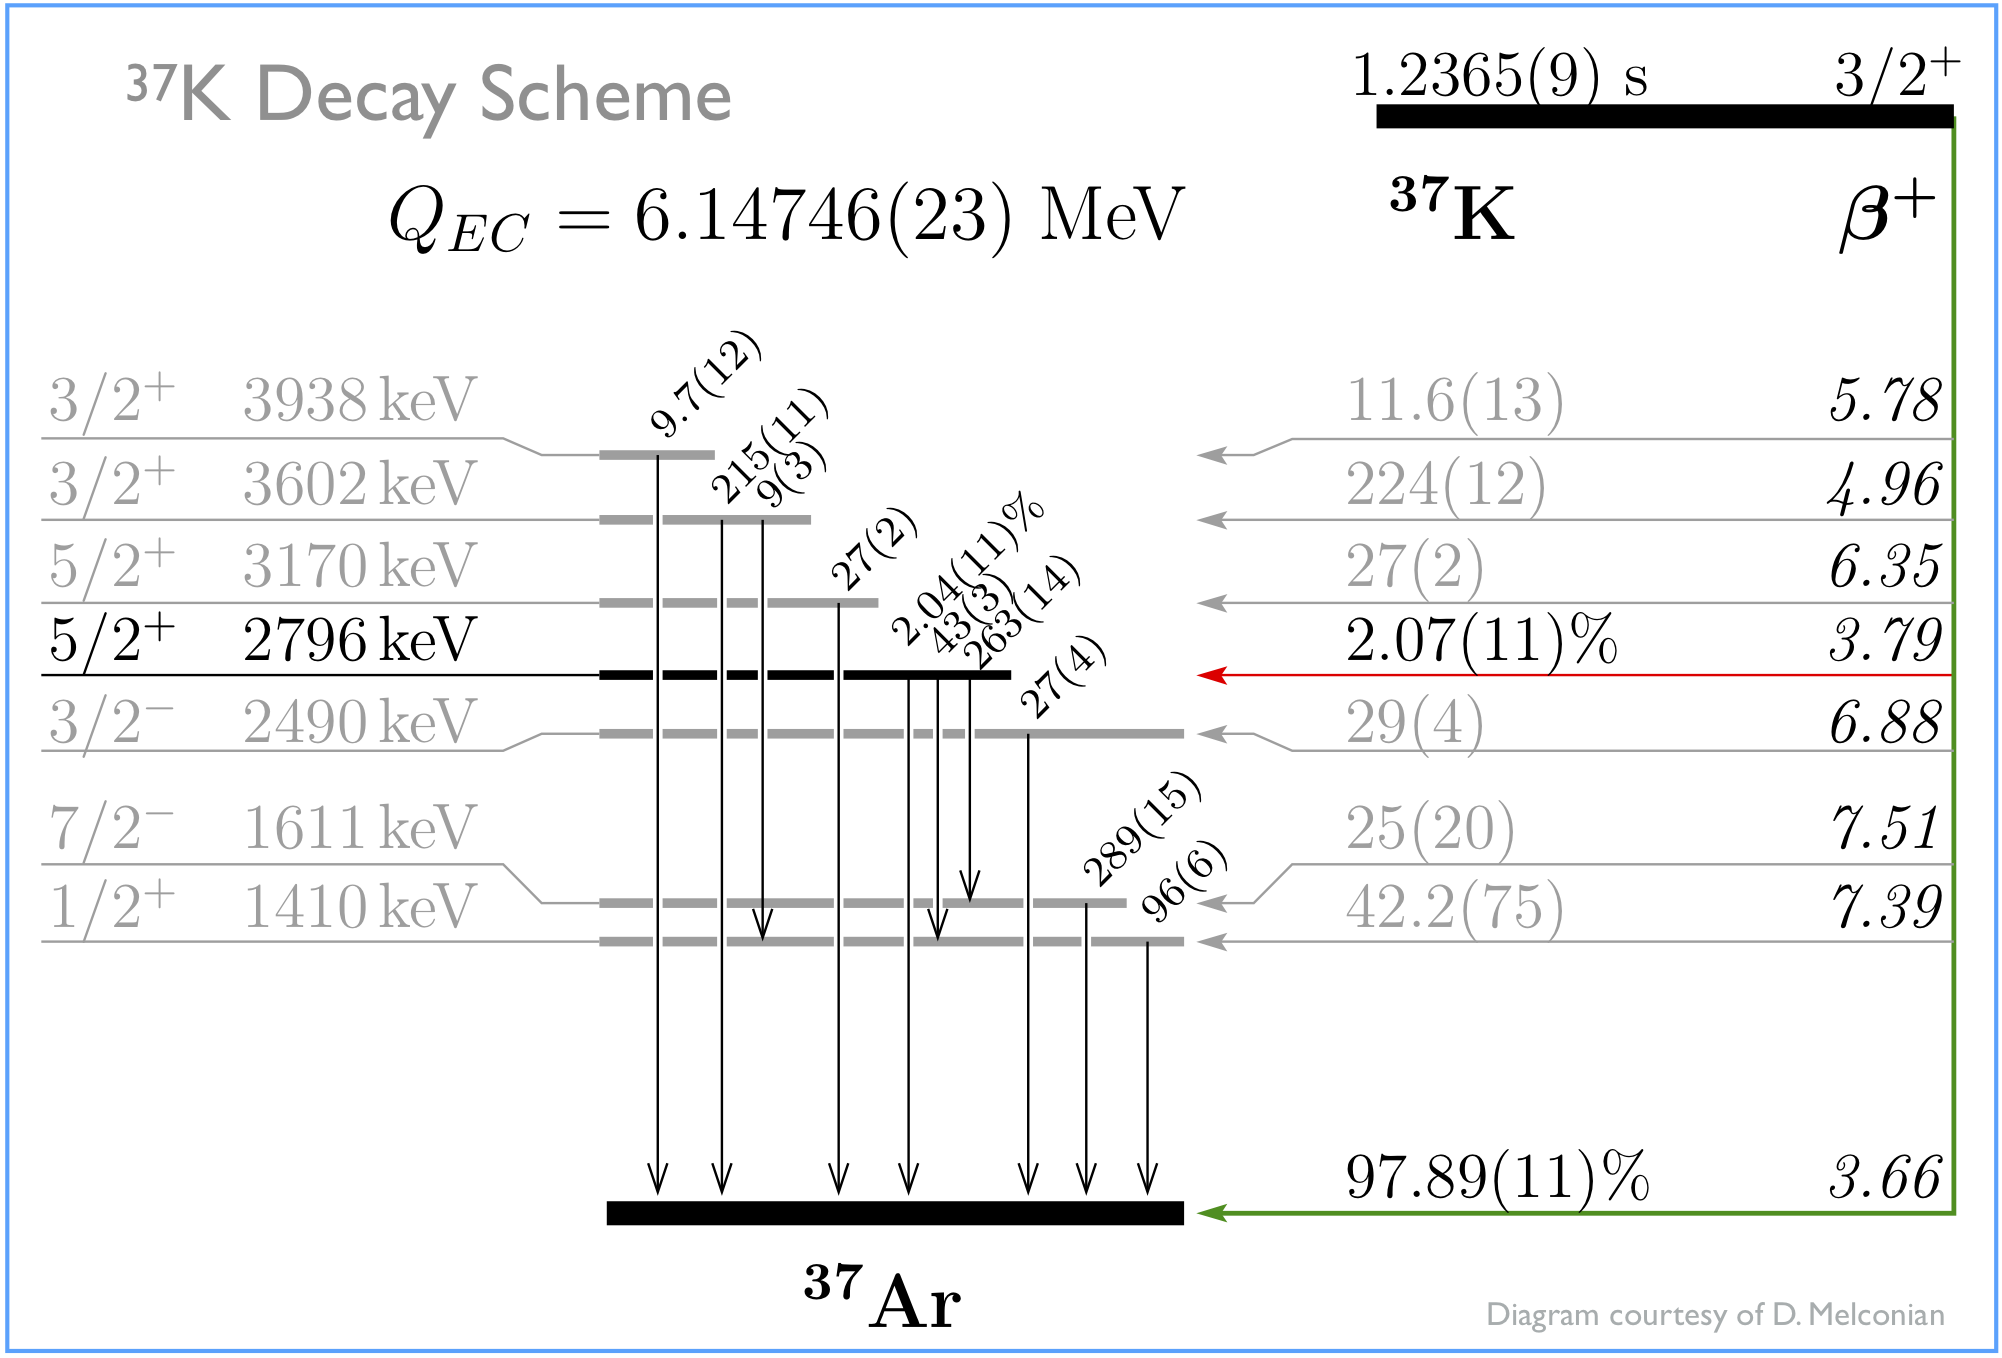
\includegraphics[width=.999\linewidth]
	{Figures/NuclearLevelDiagram.png}
	\caption{A level diagram for the decay of $\isotope[37]{K}$.}	
	\label{fig:nuclearleveldiagram}
\end{figure}


As in any decay, the angular correlations between the emerging daughter particles provide a rich source of information about the type of interaction that produced the decay.  
This particular decay involves a set of `mirror' nuclei, meaning that the nuclear wavefunctions of the parent and daughter are identical up to their isospin quantum number and corresponding electrical charge.  Because the two wavefunctions are so similar, effects to the decay from nuclear structure corrections can be kept to a minimum, and it is therefore possible to place especially strong constraints on the size of the theoretical uncertainties associated with the decay.  \aside[color=bluetodo]{Is it definitely true that the nuclear structure corrections are *smaller*?  Or is it just that they're better understood?}


%As a result, observations of this particular decay can be used to place especially strong constraints on 
%This property allows us to place strong constraints on the size of the theoretical uncertainties for this decay process within the Standard Model.  

%\note{ ``Of particular interest is the decay process: $^{37}\textrm{K} \rightarrow \,^{37}\textrm{\!Ar} + \beta^{+} + \nu_e$.  Among other useful properties, this is is a `mirror' decay, meaning that the nuclear wavefunctions of the parent and daughter are identical up to their isospin quantum number.  
%%the number of protons in the parent nucleus (19) is equal to the number of neutrons in the daughter, and the number of neutrons in the parent (18) is equal to the number of protons in the daughter.  
%This property allows us to place strong constraints on the size of the theoretical uncertainties for this decay process within the Standard Model.   %We further exploit this property by noting that both the $^{37}\textrm{K}$ parent and the $^{37}\textrm{\!Ar}$ daughter have nuclear spin $I=3/2$, a fact which is key to this experiment.
%''}


%\note{Talk about how great \isotope[37]{K} is for what we're doing with it.  Also, drop all the math-numbers to support those assertions.  Reference the level diagram within the text!}

\note{Also, 37K is a really nice isotope for this, because 
%98\% + 2\%, 
%also because it's a mirror decay, 
%also because it's an alkali.  Also-
%also, 
its big $\Abeta$ value means we have a big thing to multiply any $\bFierz$ value there might be when we construct the superratio asymmetry to eliminate systematics.}

%\missingfigure{This thing is going to need a nuclear level diagram for 37K.  Also, 37K is a really nice isotope for this, because 98\% + 2\%, also because it's a mirror decay, also because it's an alkali.  Also-also, its big $\Abeta$ value means we have a big thing to multiply any $\bFierz$ value there might be when we construct the superratio asymmetry to eliminate systematics.}


%\section{Exotic Couplings}
%%	In particular, we're interested in so-called scalar and tensor couplings within the nuclear weak force. Standard model beta decay involves only vector and axial-vector couplings, combined with a ``$(V-A)$'' handedness (left-handed).  



%%%% --- * --- %%%%	
\section{The Shake-off Electron Spectrum}
\label{section:soe_intro}
Although the beta decay process is primarily concerned with the emission of beta particles (electrons or positrons) from a Weak interaction that occurs within the nucleus, it is common for one or more \emph{orbital} electrons to also be lost in the process.  Although beta particles are emitted over a continuous energy spectrum, they commonly carry several MeV of kinetic energy.  By contrast, an atomic electron that becomes unbound in this process is likely to only carry a few eV of kinetic energy, and we say that they are `shaken' off.  

We will amend Eq.~\ref{eq:ourdecay} to reflect the presence of $N$ such `shake-off electrons' (SOEs) within each decay event, as
\bea
^{37}\textrm{K} &\rightarrow& \,^{37}\textrm{\!Ar}^{(N-1)+} + \beta^{+} + \nu_e + N \, e_{\textrm{SO}}, 
\label{eq:ourdecay_withsoe}
\eea
\aside{Do I want to re-assign N somehow so the notation works better?}
where it is clear that, since the parent $^{37}\textrm{K}$ atom was electrically neutral before its decay by $\beta^+$ emission, the daughter $^{37}\textrm{\!Ar}$ will initially have an `extra' orbital electron (and therefore a negative net charge) if no electrons are shaken off.  We also note that it is common for multiple SOEs to be created in a given decay event.  

A further consideration is that the outer electron in an $^{37}\textrm{\!Ar}^{-}$ ion is \emph{not bound},~\aside[color=bluetodo]{cite someone!!  I don't know who.} and in an electric field such as is present within our experimental chamber, this outer electron is removed immediately to be accelerated through the field, leaving behind a neutral $^{37}\textrm{\!Ar}$ atom.  Although this is in principle a different physical loss mechanism, we will refer to unbound electrons resulting from either process as SOEs.  

It is useful to consider the energy spectrum of these shake-off electrons.  The most straightforward component of the SOE energy spectrum arises from the electrons that are lost immediately following decay, and we take these to initially have 0eV in kinetic energy.  

For the shake-off electrons arising from the Weak process itself, the initial energy spectra for SOEs originating in a particular orbital shell can be estimated according to the procedure outlined by Levinger~\cite{Levinger}.  The strategy is to assume that the sudden approximation holds, and simply calculate the overlap in electron wavefunctions between the initial and final states, where the final state may be either an outgoing electron or one bound within the atom.  Analytic expressions can be obtained if the atom is treated as being hydrogenic -- an excellent approximation here, as $^{37}\textrm{K}$ is an alkali.  

Unfortunately, this treatment cannot determine the fractional contribution of each orbital to the total, nor can it determine the \emph{number} of electrons likely to be removed in a single decay event.  The implications of the SOE energy spectrum to the present experiment are discussed further in Section~\ref{sec:tof_bg} 

\note[color=bluetodo]{In the end, we used $(0.09)*(\textrm{0eV}) + (0.91)*(0.85*(\textrm{4S}) + 0.15*(\textrm{3P}))$.  But I say that in the other section.  Also, John used Eq.20 for the 4S, and Eq.24 for the 3P.}
\note{Comment on how well this matches our data?  Somehow?}

%\note{Should I talk about the distribution of how many SOEs come off in a decay?  I have measurements of the recoil charge distribution, which is related but not really the same thing.  From a theoretical POV, I don't know how many get shaken off.  Thankfully, it doesn't matter very much in the end.}

% !TEX root = ../thesis_main.tex
%
%
%%% 
\begin{figure}[h!!t]
	\centering
	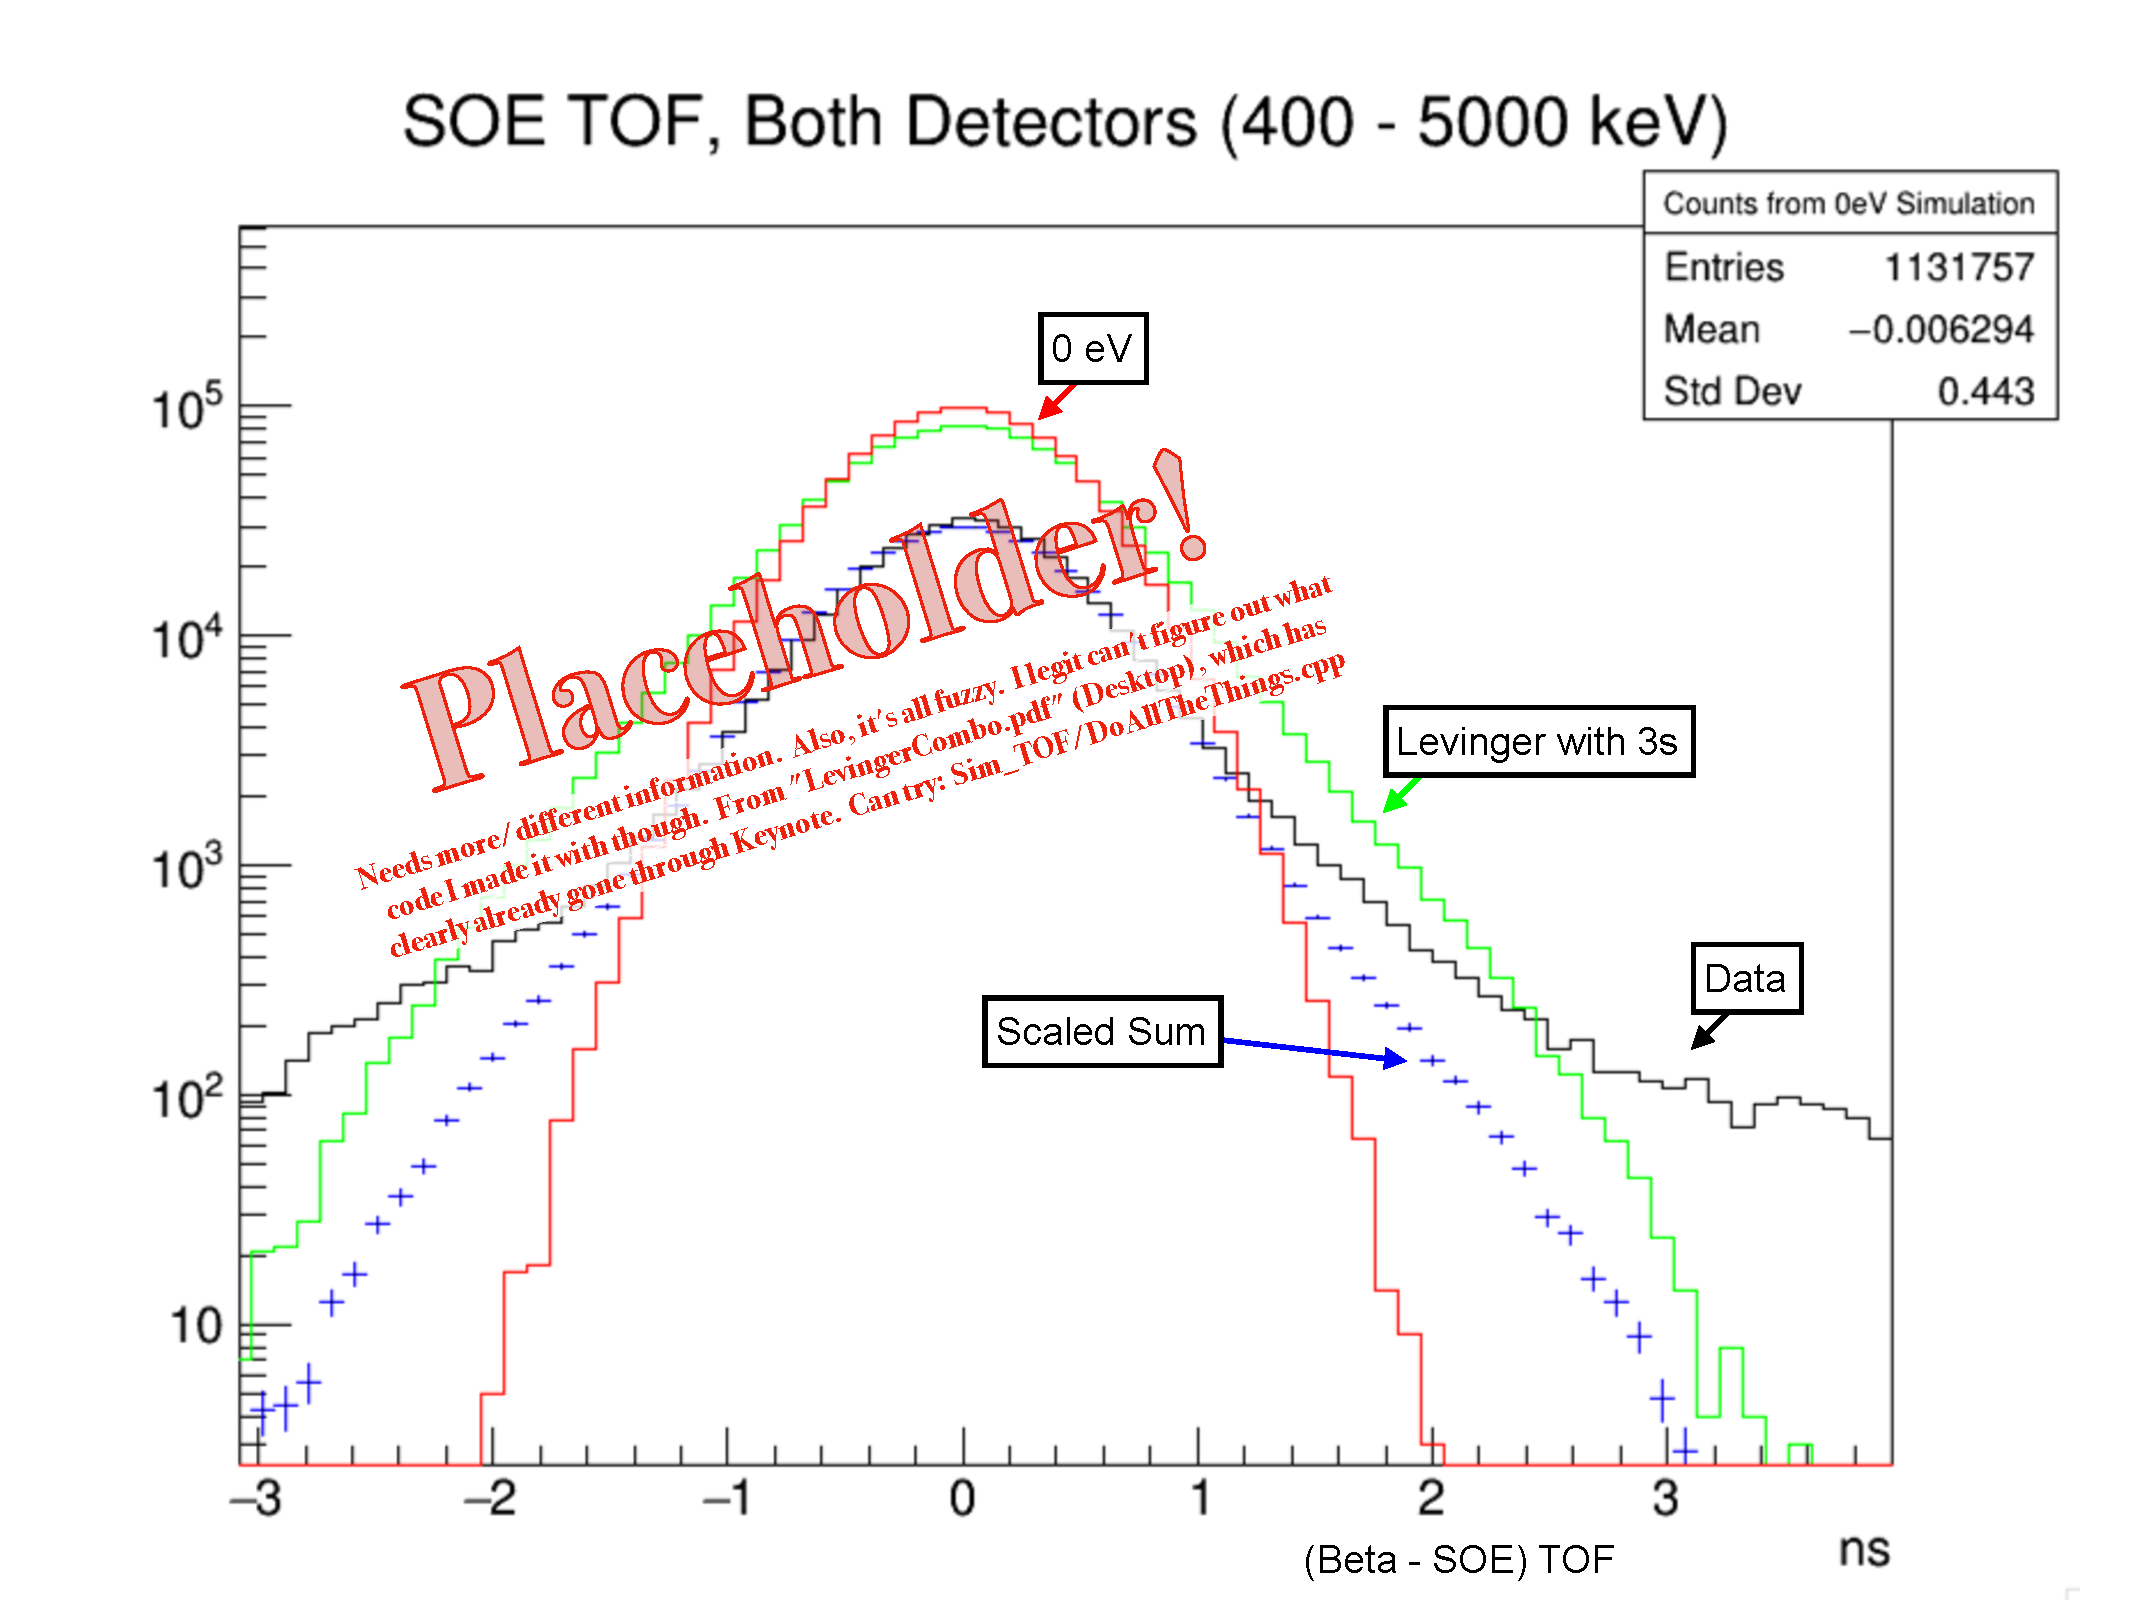
\includegraphics[width=.999\linewidth]
	{Figures/Levinger_SOETOF_prelim.pdf}
	\note{Maybe just kill this picture?  At least reference it in the text somewhere.}
	\caption[Levinger TOF]{Shake-off electron TOF (w.r.t. beta TOA) spectrum, showing how the spectrum is different if one includes different sets of initial electrons to be shaken off.  I forget why some of them have 0 eV.  Maybe those are the ones from the $\isotope[37]{Ar}^+$. ... Levinger TOF spectra for some different sets of SOE initial orbitals before shake-off.  (At least that's what it's supposed to be, after I fix the picture).  It's reconstructed event-by-event with beta times-of-flight that would pass some basic `good event' cuts.  Anyway, it turns out, it doesn't much matter what orbitals you lose SOEs from.  That's nice.  In the end, I used 85+15.  \comment{(Need to re-plot this.)} }	
	\label{fig:levinger_TOF}
\end{figure}




%%%% --- * --- %%%%
\FloatBarrier  % This will have to go away later.
\section{Fierz Interference -- The Physical Signature}
\label{signature_chapter}
%\note[color=jb]{JB:  ``I doubt I will have further useful comments on the Ch. (((this chapter))) as they are now.'' }
	The physical effects resulting from the presence of scalar or tensor couplings include a small perturbation to the energy spectrum of betas produced by radioactive decay.  

%\missingfigure{I need that simulated picture of the different beta energy spectra, with different values of $\bFierz$.}
\note[color=jb]{JB on that missing figure that I've now put in:    ``A dependence of Abeta on beta energy is also introduced.
\\
UCNA fits energy spectrum and Abeta[Ebeta] simultaneously now."
}

%\section{Present Limits}
%	A bit about other people's physics.

\note{The point is, the presence of either scalar or tensor interactions will produce a $\bFierz$ term in the decay PDF.  It has other effects on the PDF, but those come in at higher-order in the tiny scalar and tensor couplings.  So, the Fierz term would be by far the biggest thing that changes in the PDF.  The PDF describes the energy and momentum of the outgoing beta w.r.t. a variety of other things.  Notably, we can write an elegant-ish description of beta momentum w.r.t. nuclear polarization direction, and ignore the neutrino completely after integrating over it.  We have a PDF in beta \emph{direction} (w.r.t. polarization), and beta \emph{energy}.  To lowest order (and lowest order is best order) the distribution w.r.t. polarization direction doesn't change, but the distribution w.r.t. energy does change.  Or ... something?  The point is, it makes a change in the beta energy spectrum.  This change is most pronounced at low energies, because the Fierz term is scaled by $(1/\Ebeta)$.  However, the asymmetry is also a function of $\Ebeta$.  A different function of $\Ebeta$.  In fact, it is scaled by $(\pbeta/\Ebeta)$ within the PDF, which is distinctly different than $\bFierz$.  So, one might ask what effect a $\bFierz$ term would produce on a constructed asymmetry spectrum.  ....This explanation has gone way off track.}

\note{Here's a reference to the picture that shows the result of a non-zero $\bFierz$ term.  It's Fig.~\ref{fig:FierzSignature}.}

\begin{figure}[h!!t]
	\centering
	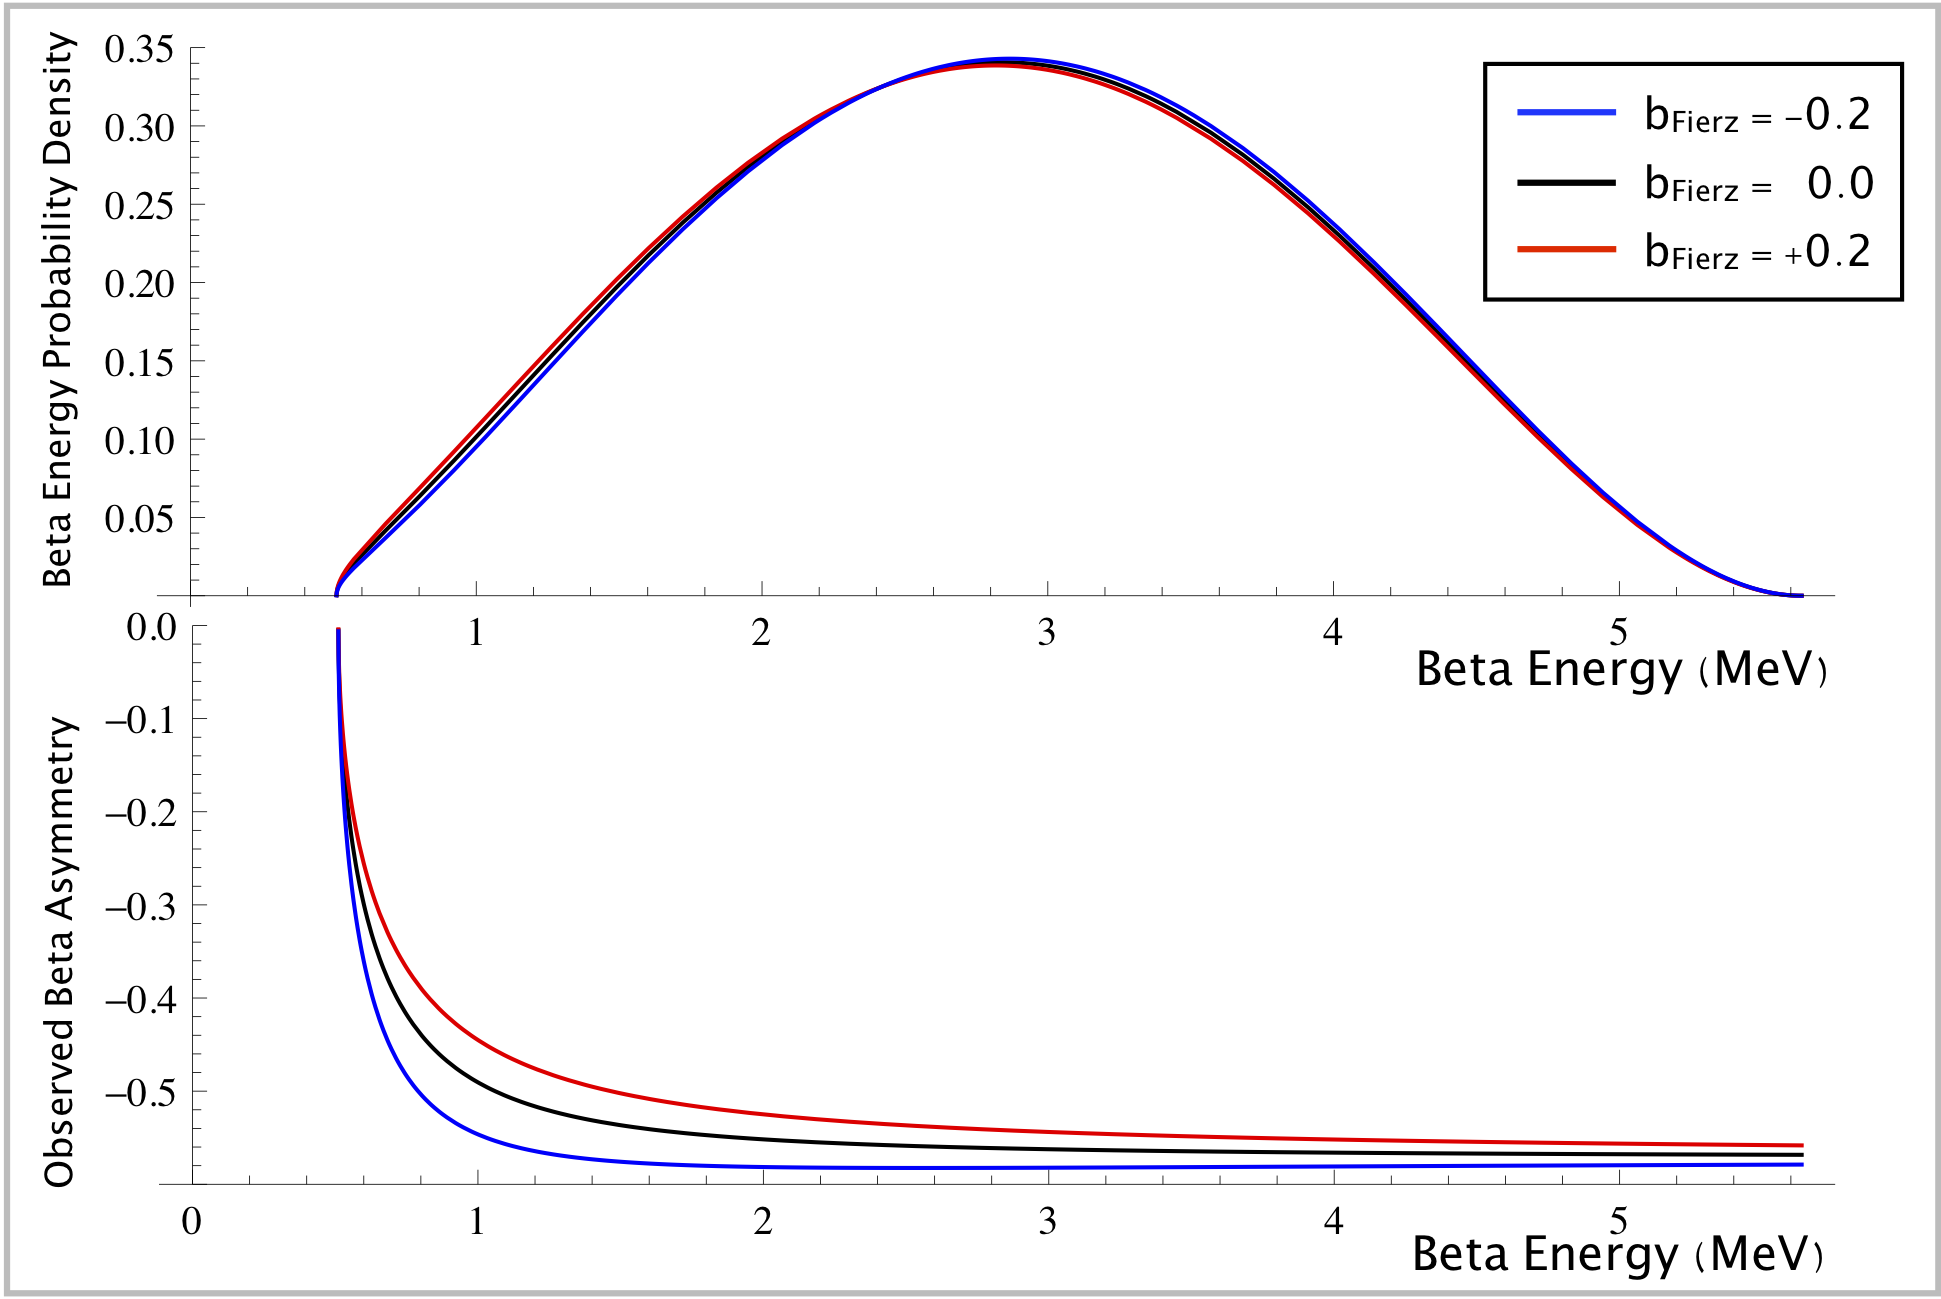
\includegraphics[width=.999\linewidth]
	{Figures/Fierz_Signature.png}
	\caption{Here's why it's better to extract $\bFierz$ from an asymmetry, in this case.}	
	\label{fig:FierzSignature}
\end{figure}


\section{On the Superratio, the Supersum, and the Constructed Asymmetry}
\note[color=jb]{JB:  You need to at some point say that the supersum is the beta energy spectrum.  There are experiments trying to do this method better, but they are very difficult.  UCNA published a combined energy spectrum and Abeta[Ebeta] analysis on the neutron in March 2020~\cite{NeutronbFierz_March2020}.
\\...\\
MJA:  I can't help but also notice the follow-up article from September 2020~\cite{Saul2020}.  Ugh. 
}

%\\*
The data can be combined into a superratio asymmetry.  This has the benefit of causing many systematics to cancel themselves out at leading order.  It also will increase the fractional size of the effects we're looking for.  This can be shown by using math.  

%\\*
Not all systematics effects are eliminated.  We'll want to be careful to propagate through any effects that are relevant.  Using the superratio asymmetry as our physical observable makes this process a bit messier for the things that don't cancel out, but it's all just math.  
%\\*
Some other groups have performed similar measurements using the supersum as the physical observable.  There are pros and cons to both methods.  I can show, using a back-of-the-envelope calculation, that for this particular dataset, the superratio asymmetry method produces a better result.  


